\documentclass[12pt]{article}
\usepackage[utf8]{inputenc}
\usepackage{graphicx}
\usepackage[a4paper,width=150mm,top=25mm,bottom=25mm]{geometry}

\title{Testing Policy}
\author{Ctrl Alt Defeat}

\begin{document}
\begin{titlepage}
    \centering



    \vspace{2cm}
    \hrulefill\\
    \vspace{1cm}
    {\Huge\bfseries SRS Documentation v3.0}

    \vspace{1cm}

    {\Large Software Requirements Specification Document for\\Domain Pulse}\\
    \vspace{1cm}
    \hrulefill\\

    \vfill

    {\large Ctrl Alt Defeat}

    \vspace{1cm}

    {\large 2023/07/31}\\
    %    \vspace{1cm}
    %    \vspace{1cm}
    %    
\includegraphics[width=10cm]{../../Images/dpLogo.png}
    %    \vspace{1cm}\\
    %    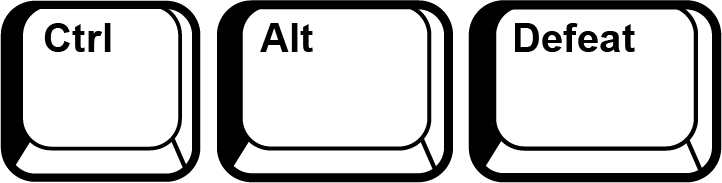
\includegraphics[width=6cm]{../../Images/cadLogo.png}

\end{titlepage}


\tableofcontents
\newpage

\newpage
\section{Quality Requirements Testing}
\subsection{Usability}
\subsection{Security}
\subsection{Performance}
\subsection{Scalability}
\subsection{Modifiability}

\newpage
\section{Code Coverage}
Any commit made to a branch causes automated tests to be run on the codebase of that branch, thereafter the code coverage of said branch is calculated.
Any branch being merged via pull request into the development branch (dev) needs to have the coverage of changes to the codebase to match or better the coverage of the development branch.
Furthermore, the coverage of the newly commited code (ie: patch) must match or exceed the coverage percentage of the project.
This ensures that the coverage of the codebase is never decreasing, and that sufficient testing is being done on the codebase.
Furthermore any time the development branch is merged into the master branch, the coverage of the development branch must match or be higher than that of the master branch, ensuring an increasing coverage and sufficient testing.

\newpage
\section{Choice of testing tools/frameworks}
\subsection{Frontend Testing}
For our frontend testing frameworks and tools we decided to use the following:
\begin{itemize}
    \item \textbf{Karma and Jasmine} - Jasmine is the testing framework that is used to write actual tests and Karma is the test runner that executes the tests. Karma is run from a CLI(Command Line Interface) and it will open up a browser window and run the tests in that browser. Karma will then report the results of the tests back to the CLI. Karma and Jasmine are recommended by Angular which is what our frontend is primarily built upon and they are the most popular testing frameworks for Angular applications.
\end{itemize}



\end{document}